\chapter{Teori}\label{Teori}

<<<<<<< HEAD
\section{Dijkstras Algoritme}

Dijkstras algoritme er en algoritme til at finde den korteste vej fra et bestemt punkt til et andet punkt. Disse punkter kan bland andet repræsentere den korteste vej mellem to forskellige byer. Dijkstras er en grådig algoritme, da den finder den mindste længde først og fortsætter således.\cite{DMATBOGEN}
Dijkstras algoritme finder den korteste rute mellem 2 forskellige punkter i en simpel ikke-orienteret vægtet graf. Nedenfor er der en graf, med forskellige punkter {A, B, C, D, E, Z}. Hvis man skal fra punkt A til Z, så starter man ved A og derfor initialiseres A til at være 0. Algoritmen virker således, at alle punkter er uendeligt udover det punkt man befinder sig på. Algoritmen tager punkt fra punkt, så den starter med at se de grene som A har disse er |AB| = 4 og |AC| = 2. Her fra kan algoritmen ikke se videre end B og C. Den ser altid på det mindste tal, og derfor tager den |AB| = 4 og |AC| = 2, da begge disse tal er mindre end uendeligt. Herefter ser den efter hvilket af de nuværende tal som er mindst, hvilket er 2. Så derfor vælger den C som sit næste punkt. Algoritmen finder nu de næst tætteste punkt, ved at addere alle de tidligere ruter, som har den korteste rute fra A til det næste sæt af punkter. Her ser algoritmen ud fra C og hvilke grene C har. Dette er |CB| |CD| |CE|, dog er længden altid fra A, så derfor er længden fra A til E 12 da 2+10 = 12. Længden til B er nu blivet 3, da algoritmen ser på den mindste rute, så A til B er 3, da 2+1 = 3. Således fortsætter algoritmen indtil den rammer Z.\cite{DMATBOGEN}

\begin{lstlisting}[language=c][caption={Dijkstras angivet som eksempel i pseudo-kode},label={lst:DijsktrasPseudo1}]
	procedure Dijkstras(G: weighted connected simple graph, with all weights positive)
{G has vertices a = V0, V1, ....... Vn = z and lengths w(Vi, Vj) where w(Vi,Vj) = infinity if{Vi, Vj} is not an edge in G}
for (i = 1 to n)
	L(Vi) = infinity
L(a) = 0
S = NULL
{ the labels are now initialized so that the label of a is 0 and all other labels are infinity, and S is the empty set }
while (z does not belong to S)
	u = a vertex not in S with L(u) minimal
	S = S U {u}
	for (all vertices v not in S)
		if (L(u) + w(u, v) < L(v) then L(v) = L(u) + L(u, v))
		{this adds a vertex to S with minimal label and updates the labels of vertices not in S}
return (L(z)) {L(z) = length of a shortest path from 	a to z}
\end{lstlisting}

\section{A* Algoritmen}
=======
\section{A* Algoritmen}\label{A-Algoritmen}
>>>>>>> 1d857fcaf189d131f19ed917d91e5cdb2bb39ea6
Primært når det kommer til belægning af en dynamisk rute, foregår det ved at en enhed fortsætter hen i mod et mål indtil den når en forhindring. Dette er et ekstremt simpelt bevægelsesmønster og indebærer in vis in-effektivitet. Rent retorisk kunne man stille spørgsmålet om det ikke ville være smartere at planlægge en rute før man overhovedet bevæger sig.

A* er en algoritme til at beregne den korteste rute baseret på en række heuristiske datasæt. A* får input igennem en brugerlavet graf der indeholder en række datasæt for at algoritmen kan fungere.  Først har vi distancen fra punkt til punkt, eksempelvis punkt 'A' til punkt 'B' som vi kalder for f.eks. \textbf{'H'} og dernæst har vi et datasæt \textbf{'G'} der indeholder bekostningen for at flytte fra en kant til en anden, denne variabel er bestemt på forhånd. Et virkelighedseksempel kunne være at man vil over på den anden side af en sø, så har man så muligheden for at svømme direkte eller gå uden om og det koster f.eks. 2 gange så meget at bevæge sig direkte igennem søen. Dette er givet ved \textbf{'G'}, hvor som sagt \textbf{'H'} er den ultimative korteste længde til det bestemte slutpunkt. \textbf{'H'} fungerer desuden for hvilket som helst punkt i et system og angiver \textit{altid} den korteste vej til slutpunktet uanset forhindringer. Det skal også nævnes at \textbf{'H'} ikke er påvirket af bevægelsesbekostningen, til at starte med, som \textbf{'G'} angiver, dette kommer først senere. Til sidst har vi \textbf{'F'} der er en samenlagt værdi af både \textbf{'H'} og \textbf{'G'}. Dette gælder kun for hver kasse der flyttes til, hvori \textbf{'H'} er angivet ved kassen man flytter tils \textbf{'H'} værdi. Det kan vises således i formlen \ref{eq:A*}:
\begin{equation} \label{eq:A*}
F(n) = G(n) + H(n)
\end{equation}

En måde man kan visualisere A* på er f.eks. med et gitter-system som set i figur \ref{fig:AKvadrat1}. Her kan vi se at vi har et start punkt (grøn) og et slutpunkts (blå). De kasser vi ikke kan bevæge os igennem er de røde kasser. Figuren angiver ingen heuristiske datasæt endnu.

\begin{figure}[ht!]
\begin{adjustbox}{width=1.2\textwidth,center=\textwidth}
\label{fig:AKvadrat1}
\centering
\includegraphics[width=1.2\textwidth]{Pictures/Teoriafsnit/Figurfiler/Grid2.png}
\end{adjustbox}
\caption{A* gitter-system}
\end{figure}

Ud fra figuren kan vi begynde os at forestille hvordan A* fungerer. Når man bevæger sig fra kasse til kasse laver man 2 lister til at holde styr på hvor brikken har været. En liste til at holde styr på hvilke kasser man ikke har besøgt endnu og en liste der holder styr på hvilke man \textbf{har} besøgt. Når man flytter brikken skal man derfor angive hvilken kasse der nu skal på \textit{besøgt} listen. Derfor som nævnt skal vi bruge information om hvor meget \textbf{'G'} koster. Brikken skal nu til at flytte sig for at komme til slutpunktet. Dette kunne f.eks. være 10 point for at flytte sig i hvilken som helst retning, men man kunne også sagtens angive at diagonal bevægelse ville koste 12 point. Dvs. at ruten ændrer sig til måske ikke at være så direkte som den ellers kunne have været.

Der findes flere metoder man kan anvende A* på og en af dem vises her.
Det vises her i den lille bid af pseudo-kode i figur \ref{lst:A*pseudo1}
\begin{lstlisting}[language=c][caption={Pseudo-kode af lister i A*},\label{lst:A*pseudo1}]
	class A_Star
	{
		List<int> nodeIdentifierVisited = new List<int> { 7, 8, 9 , 10, 11, 12, 13, 14, 21, 23, 24, 28, 29, 30, 31, 32};

		Expand to new node from previous and move
		Queue frontQueue = new Point();

		when Point is acknowledged to move
		change new Point to become Visited = true;

		while(new Point == Visited)
		{
			move Point to nodeIdentifierVisited
		}
	}
\end{lstlisting}

Som set i figur \ref{fig:AKvadrat1} har vi vores liste givet ved kassernes nummerering. Nummereringen kører fra venstre mod højre én række ad gangen. Vi angiver at det tager 10 point af gå lodret og vandret én kasse ad gangen og 12 point at gå diagonalt. I figur \ref{fig:AKvadrat2} kan vi nu se de heuristiske datasæt angivet fra startpunktet (grøn). Hver enkel kasse omkringliggende startpunktet har deres \textbf{'H'} værdi angivet med lys-lilla tekst og bevægelsesomkostningen \textbf{'G'} fra startpunktet til kassen angivet i blå tekst.

\begin{figure}[ht!]
\begin{center}
\includegraphics[width=1.00\textwidth]{Pictures/Teoriafsnit/Figurfiler/Grid3.png}
\end{center}
\label{fig:AKvadrat2}
\caption{A* der viser bekostning af bevægelse fra startpunkt (grøn) til omkringliggende kasser ('G') angivet med blå farve samt 'H' angivet med lys-lilla}
\end{figure}

Nu udregnes \textbf{'F'} værdien så f.eks. hvis vi går fra kasse 14 (startpunktet) til 15 skal vi lægge 10 (\textbf{'G'}) og 8 (\textbf{'H'}) sammen. Dette gør vi så for alle omkringliggende kasser for startpunktet. Dernæst går man til den laveste \textbf{'F'} værdi og gør helt det samme som før, derudover flyttes den nye kasse man står på til \textit{besøgt} listen. Noget man skal være opmærksom på her er at man stadig skal sammenligne bevægelsesomkostningen fra den tidligere kasse